%% abtex2-modelo-artigo.tex, v-1.9.2 laurocesar
%% Copyright 2012-2014 by abnTeX2 group at http://abntex2.googlecode.com/ 
%%
%% This work may be distributed and/or modified under the
%% conditions of the LaTeX Project Public License, either version 1.3
%% of this license or (at your option) any later version.
%% The latest version of this license is in
%%   http://www.latex-project.org/lppl.txt
%% and version 1.3 or later is part of all distributions of LaTeX
%% version 2005/12/01 or later.
%%
%% This work has the LPPL maintenance status `maintained'.
%% 
%% The Current Maintainer of this work is the abnTeX2 team, led
%% by Lauro César Araujo. Further information are available on 
%% http://abntex2.googlecode.com/
%%
%% This work consists of the files abntex2-modelo-artigo.tex and
%% abntex2-modelo-references.bib
%%

% ------------------------------------------------------------------------
% ------------------------------------------------------------------------
% abnTeX2: Modelo de Artigo Acadêmico em conformidade com
% ABNT NBR 6022:2003: Informação e documentação - Artigo em publicação 
% periódica científica impressa - Apresentação
% ------------------------------------------------------------------------
% ------------------------------------------------------------------------

\documentclass[
	% -- opções da classe memoir --
	article,			% indica que é um artigo acadêmico
	11pt,				% tamanho da fonte
	oneside,			% para impressão apenas no verso. Oposto a twoside
	a4paper,			% tamanho do papel. 
	% -- opções da classe abntex2 --
	%chapter=TITLE,		% títulos de capítulos convertidos em letras maiúsculas
	%section=TITLE,		% títulos de seções convertidos em letras maiúsculas
	%subsection=TITLE,	% títulos de subseções convertidos em letras maiúsculas
	%subsubsection=TITLE % títulos de subsubseções convertidos em letras maiúsculas
	% -- opções do pacote babel --
	english,			% idioma adicional para hifenização
	brazil,				% o último idioma é o principal do documento
	sumario=tradicional
	]{abntex2}


% ---
% PACOTES
% ---

% ---
% Pacotes fundamentais 
% ---
\usepackage{lmodern}			% Usa a fonte Latin Modern
\usepackage[T1]{fontenc}		% Selecao de codigos de fonte.
\usepackage[utf8]{inputenc}		% Codificacao do documento (conversão automática dos acentos)
\usepackage{indentfirst}		% Indenta o primeiro parágrafo de cada seção.
\usepackage{nomencl} 			% Lista de simbolos
\usepackage{color}				% Controle das cores
\usepackage{graphicx}			% Inclusão de gráficos
\usepackage{microtype} 			% para melhorias de justificação

\usepackage{amsmath} 			% Equações
\usepackage{graphicx}
\usepackage{caption}
\usepackage{subcaption}
\usepackage{tikz}
 
% ---
		
% ---
% Pacotes adicionais, usados apenas no âmbito do Modelo Canônico do abnteX2
% ---
\usepackage{lipsum}				% para geração de dummy text
% ---
		
% ---
% Pacotes de citações
% ---
\usepackage[brazilian,hyperpageref]{backref}	 % Paginas com as citações na bibl
\usepackage[alf]{abntex2cite}	% Citações padrão ABNT
% ---

% ---
% Configurações do pacote backref
% Usado sem a opção hyperpageref de backref
\renewcommand{\backrefpagesname}{Citado na(s) página(s):~}
% Texto padrão antes do número das páginas
\renewcommand{\backref}{}
% Define os textos da citação
\renewcommand*{\backrefalt}[4]{
	\ifcase #1 %
		Nenhuma citação no texto.%
	\or
		Citado na página #2.%
	\else
		Citado #1 vezes nas páginas #2.%
	\fi}%
% ---

% ---
% Informações de dados para CAPA e FOLHA DE ROSTO
% ---
\titulo{Relatório de Trabalho 2 \abnTeX}
\autor{Equipe \abnTeX\thanks{\url{http://abntex2.googlecode.com/}} \and Lauro
César
Araujo\thanks{laurocesar@laurocesar.com}}
\local{Brasil}
\data{2014, v-1.9.2}
% ---

% ---
% Configurações de aparência do PDF final

% alterando o aspecto da cor azul
\definecolor{blue}{RGB}{41,5,195}

% informações do PDF
\makeatletter
\hypersetup{
     	%pagebackref=true,
		pdftitle={\@title}, 
		pdfauthor={\@author},
    	pdfsubject={Modelo de artigo científico com abnTeX2},
	    pdfcreator={LaTeX with abnTeX2},
		pdfkeywords={abnt}{latex}{abntex}{abntex2}{atigo científico}, 
		colorlinks=true,       		% false: boxed links; true: colored links
    	linkcolor=blue,          	% color of internal links
    	citecolor=blue,        		% color of links to bibliography
    	filecolor=magenta,      		% color of file links
		urlcolor=blue,
		bookmarksdepth=4
}
\makeatother
% --- 

% ---
% compila o indice
% ---
\makeindex
% ---

% ---
% Altera as margens padrões
% ---
\setlrmarginsandblock{3cm}{3cm}{*}
\setulmarginsandblock{3cm}{3cm}{*}
\checkandfixthelayout
% ---

% --- 
% Espaçamentos entre linhas e parágrafos 
% --- 

% O tamanho do parágrafo é dado por:
\setlength{\parindent}{1.3cm}

% Controle do espaçamento entre um parágrafo e outro:
\setlength{\parskip}{0.2cm}  % tente também \onelineskip

% Espaçamento simples
\SingleSpacing

% ----
% Início do documento
% ----
\begin{document}
% Retira espaço extra obsoleto entre as frases.


% ----------------------------------------------------------
% ELEMENTOS PRÉ-TEXTUAIS
% ----------------------------------------------------------

%---
%
% Se desejar escrever o artigo em duas colunas, descomente a linha abaixo
% e a linha com o texto ``FIM DE ARTIGO EM DUAS COLUNAS''.
% \twocolumn[    		% INICIO DE ARTIGO EM DUAS COLUNAS
%
%---
% página de titulo
\maketitle
\frenchspacing 
% resumo em português
\begin{resumoumacoluna}
 Conforme a ABNT NBR 6022:2003, o resumo é elemento obrigatório, constituído de
 uma sequência de frases concisas e objetivas e não de uma simples enumeração
 de tópicos, não ultrapassando 250 palavras, seguido, logo abaixo, das palavras
 representativas do conteúdo do trabalho, isto é, palavras-chave e/ou
 descritores, conforme a NBR 6028. (\ldots) As palavras-chave devem figurar logo
 abaixo do resumo, antecedidas da expressão Palavras-chave:, separadas entre si por
 ponto e finalizadas também por ponto.
 
 \vspace{\onelineskip}
 
 \noindent
 \textbf{Palavras-chaves}: latex. abntex. editoração de texto.
\end{resumoumacoluna}

% ]  				% FIM DE ARTIGO EM DUAS COLUNAS
% ---

% ----------------------------------------------------------
% ELEMENTOS TEXTUAIS
% ----------------------------------------------------------
\textual

% ----------------------------------------------------------
% Introdução
% ----------------------------------------------------------
\section*{Introdução}
\addcontentsline{toc}{section}{Introdução}


% ---------------------------------------------------------- Seção de
% explicações ----------------------------------------------------------
\section{Translação, Rotação e Redimensionamento}
Transção, Rotação e Redimensionamento são transformações lineares que podem ser
aplicadas a um ponto, linha ou qualquer forma representável por um hiperplano.
A forma original do objeto é comumente chamada de pré imagem e após as
transformações realizadas na forma ou no posicionamento do objeto é simplesmente
chamada de imagem.
Os tipos de transformações que foram supracitados possuem uma característica
entre si. Não importa a ordem de aplicação ou mesmo a intensidade dela, sempre
será possível recuperar a forma original a partir da combinação das mesmas três
transformações.

\subsection{Translação}
A operação de tranlação move cada ponto da forma em um fator constante em uma
direção específica. A forma do objeto não sofre qualquer alteração com essa
transformação, apenas o posicionamento no espaço. A translação pode ser vista e
interpretada como a adição de vetores constantes a cada ponto da forma ou como o
deslocamento do centro de coordenadas.
A ideia de se transladar um ponto de coordenadas $(x,y)$ é calcular a nova
posição $(x_0,y_0)$ onde $(x',y')=(x+x_0,y+y_0)$ onde $x_0$ e $y_0$ é a
quantidade transladada em cada eixo da coordenada ou simplesmente a nova coordenada da
origem.
Apesar de ser exibido a translação apenas para duas coordenadas esta operação
pode ser feita em qualquer número de dimensões.
A translação pode ser expressa de forma matricial. Abaixo temos a representação
para a translação de uma forma geométrica em um espaço de três dimensões. De
forma generalizada, para qualquer número de dimensões, podemos pensar na matriz
de transformação em que todos os elementos da diagonal principal possuem o
valor 1 e a última coluna com os valores da nova origem de coordenadas.

\begin{align}
Im'=T*Im\\
Im'=\begin{bmatrix}
1 & 0 & 0 & x_0\\
0 & 1 & 0 & y_0\\
0 & 0 & 1 & z_0\\
0 & 0 & 0 & 1\\
\end{bmatrix}*
\begin{bmatrix}
x\\
y\\
z\\
1\\
\end{bmatrix}
\end{align}
Na figura \ref{fig:translacao} temos o resultado da translação na imagem.

\begin{figure}
		\centering
        \begin{subfigure}[b]{0.3\textwidth}
                
\includegraphics[width=\textwidth]{imagens/ex1/imageScale1.png}
                \caption{}
                \label{fig:TransOriginal}
        \end{subfigure}%
        ~ %add desired spacing between images, e. g. ~, \quad, \qquad, \hfill etc.
          %(or a blank line to force the subfigure onto a new line)
        \begin{subfigure}[b]{0.3\textwidth}
                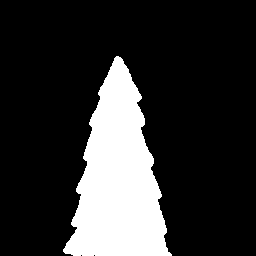
\includegraphics[width=\textwidth]{imagens/ex1/imageT1.png}
				\caption{}
                \label{fig:TransT1}
        \end{subfigure}
        ~
        \begin{subfigure}[b]{0.3\textwidth}
                
\includegraphics[width=\textwidth]{imagens/ex1/imageT2.png}
                \caption{}
                \label{fig:TransT2}
        \end{subfigure}
        ~
        \begin{subfigure}[b]{0.3\textwidth}
                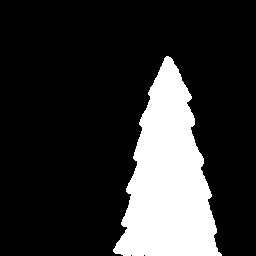
\includegraphics[width=\textwidth]{imagens/ex1/imageT3.png}
                \caption{}
                \label{fig:TransT3}       
        \end{subfigure}
        \caption{ \ref{fig:TransOriginal}. Image original
        \ref{fig:TransT1}. Imagem com translação verticalde 50 pixels
        \ref{fig:TransT2}. Imagem com translação horizontal  de 50 pixels
        \ref{fig:TransT3}. Imagem com translação vertical e horizontal de 50
        pixels}
        \label{fig:translacao}
\end{figure}

\subsection{Rotação}
A operação de rotação é uma tranformação geométrica que mapeia a posição de uma
forma em um espaço levando em consideração o ângulo desejado na transformação.
Todos os pontos da forma são rotacionados a partir de um ângulo constante em
relação ao ponto de rotação, para rotação no $\Re^2$, reta no $\Re^3$ ou
hiperplano para o $R^n$.
No $R^2$ os pontos de destino da forma podem ser calculados através das
seguintes equações:
\begin{align}
x'=cos(\theta)*(x_1-x_0)-sen(\theta)*(y_1-y_0)+x_0\\
y'=sen(\theta)*(x_1-x_0)+cos(\theta)*(y_1-y_0)+y_0\\
\end{align}
ou em termos matriciais.
\begin{align}
Im'=T*Im\\
Im'=\begin{bmatrix}
cos(\theta) & sen(\theta)\\
-sen(\theta) & cos(\theta)\\
\end{bmatrix}*
\begin{bmatrix}
x\\
y\\
\end{bmatrix}
\end{align}
Ao fazer uso da forma matricial deve-se perceber que a rotação ocorrerá somente
sobre a origem. Para contornar esta característica faz-se necessário o uso do
operador de translação, deslocando assim o ponto desejado para o centro das
coordenadas para só então realizar a rotação. Na figura \ref{fig:rotacao}
podemos ver o resultado da rotação.

\begin{figure}
		\centering
        \begin{subfigure}[b]{0.3\textwidth}
                
\includegraphics[width=\textwidth]{imagens/ex1/imageScale1.png}
                \caption{}
                \label{fig:RotOriginal}
        \end{subfigure}%
        ~ %add desired spacing between images, e. g. ~, \quad, \qquad, \hfill etc.
          %(or a blank line to force the subfigure onto a new line)
        \begin{subfigure}[b]{0.3\textwidth}
                
\includegraphics[width=\textwidth]{imagens/ex1/image30.png}
				\caption{}
                \label{fig:rot1}

        \end{subfigure}
        ~
        \begin{subfigure}[b]{0.3\textwidth}
                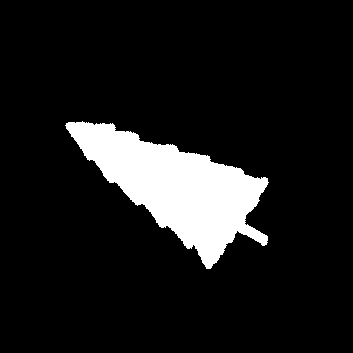
\includegraphics[width=\textwidth]{imagens/ex1/image60.png}
                \caption{}
                \label{fig:rot2}

        \end{subfigure}
        ~
        \begin{subfigure}[b]{0.3\textwidth}
                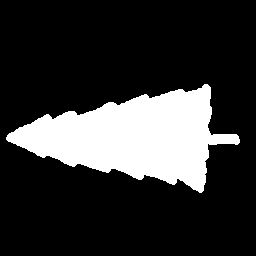
\includegraphics[width=\textwidth]{imagens/ex1/image90.png}
                \caption{}
                \label{fig:rot3}       
        \end{subfigure}
        \caption{ \ref{fig:RotOriginal}. Image original
        \ref{fig:rot1}. Imagem com rotação de 30º
        \ref{fig:rot2}. Imagem com rotação de 60º
        \ref{fig:rot3}. Imagem com rotação de 90º
        pixels}
        \label{fig:rotacao}
\end{figure}


\subsection{Redimensionamento}
O redimensionamento é uma transformação linear que aumenta ou diminue o tamanho
de uma forma em um fator constante em todas as direções da forma. Normalmente
este aumento ou redução é feita de forma uniforme, mas pode ser feita de forma
diferente em cada eixo da representação da forma. Um fator de redimencionamento
maior que 1 reflete em um aumento na imagem, menor que 1 em uma redução e um
fator igual a 1 não é feita nenhuma tranformação. É importante ressaltar que
valores menor que 0 não são válidos.
Bem como as operações de translação e rotação o redimencionamento também pode
ser representado por um produto matricial. O redimensionamento de um vetor
$\overleftarrow{v}=(x,y,z)$ por um fator $f$ resulta em um vetor
$\overleftarrow{w}=(fx,fy,fz)$, representado matricialmente por:

\begin{align}
Im'=T*Im\\
 Im' = 
\begin{bmatrix}
f_x & 0 & 0  \\
0 & f_y & 0  \\
0 & 0 & f_z  \\
\end{bmatrix}*
\begin{bmatrix}
x\\
y\\
z\\
\end{bmatrix}
\end{align}

$f_x,f_y,f_z$ são os fatores de redimensionamento para cada dimensão do vetor.

\begin{figure}
		\centering
        \begin{subfigure}[b]{0.3\textwidth}
                
\includegraphics[width=\textwidth,scale=1]{imagens/ex1/imageScale1.png}
                \caption{}
                \label{fig:RedOriginal}
        \end{subfigure}%
        ~ %add desired spacing between images, e. g. ~, \quad, \qquad, \hfill etc.
          %(or a blank line to force the subfigure onto a new line)
        \begin{subfigure}[b]{0.3\textwidth}
                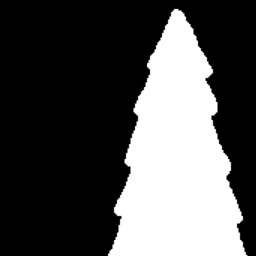
\includegraphics[width=\textwidth,scale=1]{imagens/ex1/imageScale2.png}
                \caption{}
                \label{fig:Red2}
        \end{subfigure}
        ~
        \begin{subfigure}[b]{0.3\textwidth}
  				
\includegraphics[width=\textwidth,scale=1]{imagens/ex1/imageScale3.png}
                \caption{}
                \label{fig:Red3}   
        \end{subfigure}
        \caption{ 
        \ref{fig:RedOriginal}. Image original
        \ref{fig:Red2}. Redimensionamento com fator 1.5
        \ref{fig:Red3}. Redimensionamento com fator 2
        }
        \label{fig:redimensionamento}
\end{figure}

\section{Contrate, Brilho e Gama}
As técnicas de modificação de histograma são conhecidas como técnicas ponto-a-ponto, uma
vez que o valor de tom de cinza de um certo pixel após o processamento depende apenas de seu
valor original. Dentre as principais técnicas temos o ajuste de brilho,
contraste e gama.\cite{1}

\subsection{Brilho}
O Brilho é um atributo de percepção visual no qual determina a intensidade de
energia emitida ou refletida por uma fonte, O brilho é uma característica
importante pois é ela que determina se a quantidade de luz é perceptível pelos
sensores ou pela aplicação. O ajuste de intensidade do brilho é feito a partir
da seguinte equação:
\begin{align}
Im'(x,y) = Im(x,y) + b
\end{align}
onde b é o valor de ajuste do brilho.


\subsection{Contraste}
O contrates é um atributo que permite que objetos sejam discriminados dentro de
um mesmo campo visual. Dois objetos com intensidades semelhantes são
dificilmentes distringuidos por sensores como o olho humano. O ajuste no
contraste tem como princípio aumentar a diferença de intensidade entre os
objetos.

\begin{align}
Im'(x,y) = c * Im(x,y)
\end{align}
onde c é o valor de ajuste do contraste.

\begin{figure}
\centering
		\begin{tikzpicture}[domain=0:255,scale=0.015]
		\begin{scope}                           % scope environment
			\clip  (-50,-10) rectangle (320,320);
			\draw[->] (-0,0) -- (255,0) node[above] {$x$};
			\draw[->] (0,-0) -- (0,255) node[above] {$f(x)$};
			\draw[color=red, domain=0:137] plot (\x,1.5*\x + 50) node[right] {};
			\draw[color=red, domain=137:255] plot (\x,255) node[right] {$f(x) = x$};
		\end{scope}
		\end{tikzpicture}
		\caption{Função de mapeamento com brilho=50 e contraste=1.5}
\end{figure}
~
\begin{figure}
\centering
	\begin{tikzpicture}[domain=0:255,scale=0.015]
		\begin{scope}                           % scope environment
			\clip  (-50,-10) rectangle (320,320);
			\draw[->] (-0,0) -- (255,0) node[above] {$x$};
			\draw[->] (0,-0) -- (0,255) node[above] {$f(x)$};
			\draw[color=red, domain=20:122] plot (\x,2.5 * \x - 50) node[right] {};
			\draw[color=red, domain=122:255] plot (\x,255) node[right] {$f(x) = x$};
			\draw[color=red, domain=0:20] plot (\x,0) node[right] {};
		\end{scope}           
	\end{tikzpicture}
	\caption{Função de mapeamento com brilho=-50 e contraste=2.5}
\end{figure}

\subsubsection{Gama}
O gama, assim como o ajuste de contraste é utilizado para aumentar a diferença
de intensidade entre os objetos porem de forma não linear. A regulação do gama
pode ser feita com base na seguinte função.
\begin{align}
Im'(x,y) = c * Im(x,y)^\gamma
\end{align}
onde c é um fator de correção do gama e $\gamma$ é o fator de gama. O fator de
correção é importante pois geralmente o função descrita acima retorna valores
muito altos.
\begin{figure}
\centering
		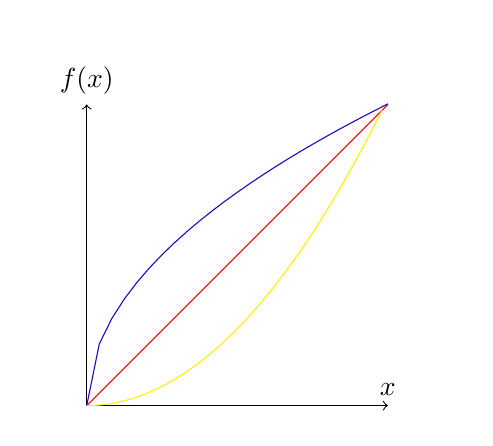
\begin{tikzpicture}[domain=0:255,scale=0.015]
		\begin{scope}                           % scope environment
			\clip  (-50,-10) rectangle (320,320);
			\draw[->] (-0,0) -- (255,0) node[above] {$x$};
			\draw[->] (0,-0) -- (0,255) node[above] {$f(x)$};
			\draw[color=red, domain=0:255] plot (\x,\x^1) node[above] { };
			\draw[color=blue, domain=0:255] plot (\x,16*\x^0.5) node[below] { };
			\draw[color=yellow, domain=0:25] plot ( 10 * \x, 0.4 * \x^2 ) node[above]{};
			
		\end{scope}
		\end{tikzpicture} 
		\caption{Função de mapeamento do gama. vermelho, azul e amarelo possuem 1,
		0,5 e 2 valores de gama respectivamente}
\end{figure}

\subsection{Filtragem no domínio da frequência}
A transformada de Fourier é uma transformação matemática que permite que funções
possam ser expressas em componentes senoidais. O somatório destas componentes
tem como resultado a função orignal. A informação de frequencia destas
componentes são muito importantes tendo em vista que com elas podemos
identificar e filtrar ruídos que atuam em frequencias conhecidas. Também pode-se
fazer a filtragem de componentes de maiores ou menores frequencias a partir de
um limiar, filtros passa-baixa e filtros passa-alta respectivamente.

Para um sinal de uma dimensão temos a seguinte equação utilizada para calcular a
transforda de fourier de $s(t)$:
\begin{align}
S(f) = \int_{-\infty}^{\infty} s(t) \cdot e^{-i 2\pi f t} dt.
\end{align}
Para duas dimensões temos a seguinte equação:
\begin{align}
\displaystyle \hat{f}(\xi_x, \xi_y)=
\displaystyle \iint f(x,y) e^{-2\pi i(\xi_x x+\xi_y y)}\,dx\,dy
\end{align}

$\xi_x$ e $\xi_y$ são as frequências calculadas sobre a imagem.
À medida que nos aproximamos da origem da transformada, imagem calculada a
partir da equação anterior, as baixas frequências correspondem aos componentes
de intensidade de variação lenta em uma imagem como mudanças suaves de
intensidade na parede ou em outras regiões uniformes da imagem.
À medida que nos distanciamos da origem da transformada, as frequências mais
altas começam a corresponder a variações de intensidade cada vez mais rápidas
como bordas de objetos e outros elementos, figura
\ref{fig:lenaOriginalEspectro}.
De acordo com as características citadas anteriormente podemos contruir as
máscaras para a filtragem  no dominio da frequencia, figura
\ref{fig:filtrosFrequencia}. Uma das características do domínio da frequência é
que a filtragem espacial pode ser realizada utilizando apenas um produto de
matrizes. O resultado da filtragem pode ser visualizado na figura.


\begin{figure}
		\centering
        \begin{subfigure}[b]{0.3\textwidth}
                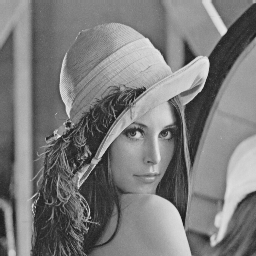
\includegraphics[width=\textwidth,scale=1]{imagens/ex2/lena.png}
                \caption{}
                \label{fig:lenaOriginal}
        \end{subfigure}%
        ~ %add desired spacing between images, e. g. ~, \quad, \qquad, \hfill etc.
          %(or a blank line to force the subfigure onto a new line)
        \begin{subfigure}[b]{0.3\textwidth}
                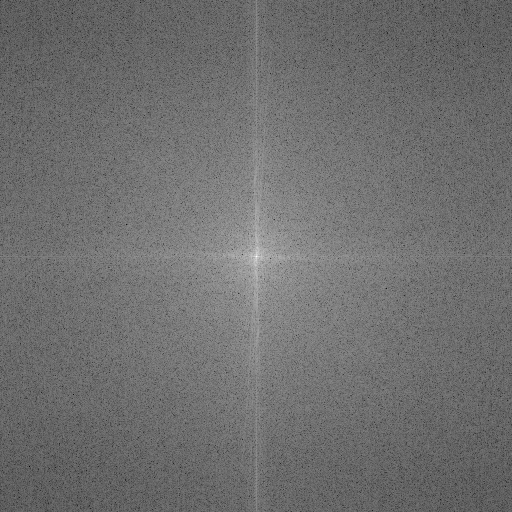
\includegraphics[width=\textwidth,scale=1]{imagens/ex2/espectroOriginal.png}
                \caption{}
                \label{fig:especOriginal}
        \end{subfigure}
       
        \caption{ 
        \ref{fig:lenaOriginal}. Image original
        \ref{fig:especOriginal}. Espectro de Fourier da imagem.
        }
		\label{fig:lenaOriginalEspectro}
\end{figure}

\begin{figure}
		\centering
        \begin{subfigure}[b]{0.3\textwidth}
                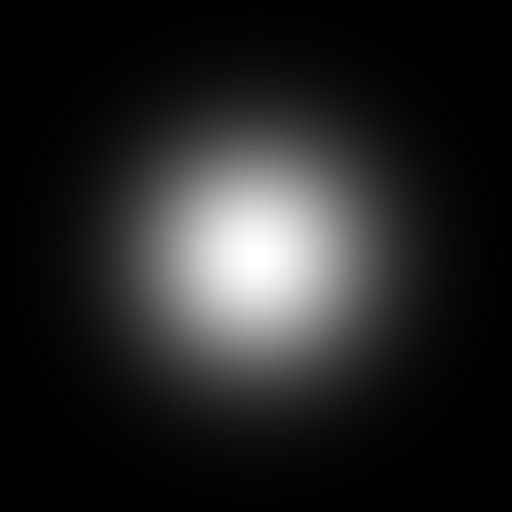
\includegraphics[width=\textwidth,scale=1]{imagens/ex2/passaBaixa.png}
                \caption{}
                \label{fig:passaBaixa}
        \end{subfigure}%
        ~ %add desired spacing between images, e. g. ~, \quad, \qquad, \hfill etc.
          %(or a blank line to force the subfigure onto a new line)
        \begin{subfigure}[b]{0.3\textwidth}
                
\includegraphics[width=\textwidth,scale=1]{imagens/ex2/passaAlta.png}
                \caption{}
                \label{fig:passaAlta}
        \end{subfigure}
       
        \caption{ 
        \ref{fig:passaBaixa}. Filtro passa baixa.
        \ref{fig:passaAlta}. Filtro passa alta.
        }
	\label{fig:filtrosFrequencia}
\end{figure}






\begin{figure}
		\centering
        \begin{subfigure}[b]{0.3\textwidth}
                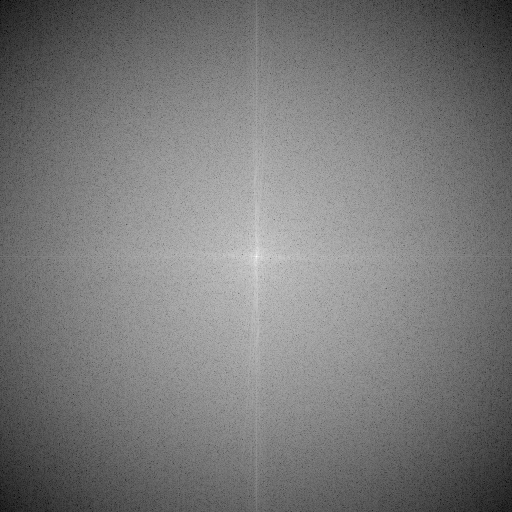
\includegraphics[width=\textwidth,scale=1]{imagens/ex2/filtradaPBSpec.png}
                \caption{}
                \label{fig:passaBaixa}
        \end{subfigure}%
        ~ %add desired spacing between images, e. g. ~, \quad, \qquad, \hfill etc.
          %(or a blank line to force the subfigure onto a new line)
        \begin{subfigure}[b]{0.3\textwidth}
                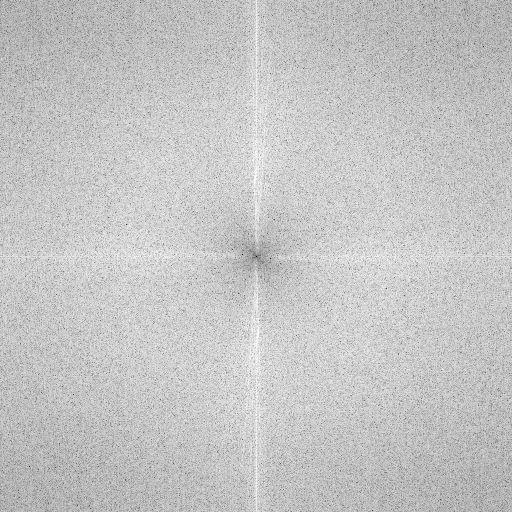
\includegraphics[width=\textwidth,scale=1]{imagens/ex2/filtradaPASpec.png}
                \caption{}
                \label{fig:passaAlta}
        \end{subfigure}
 		~      
		\centering
        \begin{subfigure}[b]{0.3\textwidth}
                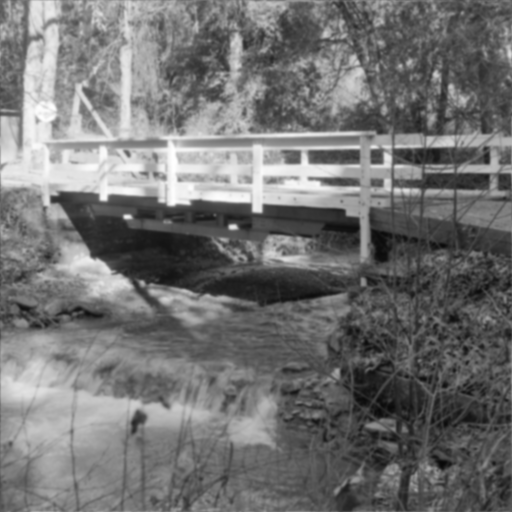
\includegraphics[width=\textwidth,scale=1]{imagens/ex2/filtradaPB.png}
                \caption{}
                \label{fig:passaBaixa} 
        \end{subfigure}%
        ~ %add desired spacing between images, e. g. ~, \quad, \qquad, \hfill etc.
          %(or a blank line to force the subfigure onto a new line)
        \begin{subfigure}[b]{0.3\textwidth}
                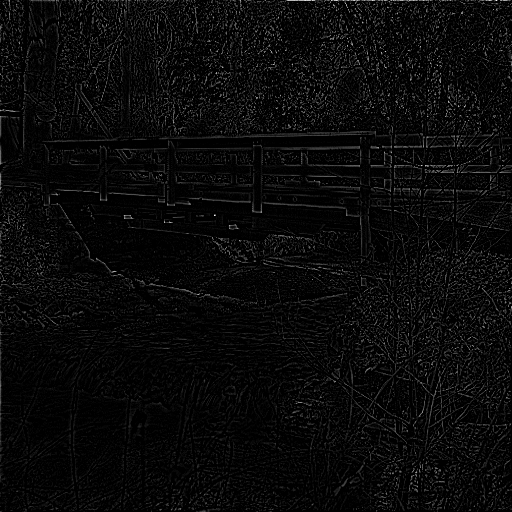
\includegraphics[width=\textwidth,scale=1]{imagens/ex2/filtradaPA.png}
                \caption{}
                \label{fig:passaAlta}
        \end{subfigure}      
       
       
       
        \caption{ 
        \ref{fig:passaBaixa}. Filtro passa baixa.
        \ref{fig:passaAlta}. Filtro passa alta.
        }
	\label{fig:filtrosFrequencia}
\end{figure}

\section{Segmentação Baseada em cores}

\subsection{Espaço de cores RGB}
An RGB color space can be easily understood by thinking of it as "all possible
colors" that can be made from three colourants for red, green and blue. If only
the red light is on, the wall will look red. If only the green light is on, the
wall will look green. If the red and green lights are on together, the wall will
look yellow. Dim the red light and the wall will become more of a yellow-green.
Dim the green light instead, and the wall will become more orange. Bringing up
the blue light a bit will cause the orange to become less saturated and more
whitish. In all, each setting of the three dimmer switches will produce a
different result, either in color or in brightness or both.

\subsection{Espaço de cores HSV}

The two representations rearrange the geometry of RGB in an attempt to be more
intuitive and perceptually relevant than the cartesian (cube) representation, by
mapping the values into a cylinder loosely inspired by a traditional color
wheel. The angle around the central vertical axis corresponds to "hue" and the
distance from the axis corresponds to "saturation". These first two values give
the two schemes the 'H' and 'S' in their names. The height corresponds to a
third value, the system's representation of the perceived luminance in relation
to the saturation.


Hue describes the shade of color and where that color it is found in the color
spectrum. Red, yellow, and purple are words that describe hue.
The next most significant aspect of color is typically the saturation,   S. The
saturation describes how pure the hue is with respect to a white reference. For
example, a color that is all red and no white is fully saturated. If we add some
white to the red, the result becomes more pastel, and the color shifts from red
to pink. The hue is still red but it has become less saturated.
Finally, a color also has a brightness.   This is a relative description of how
much light is coming from the color. If the color reflects a lot of light, we
would say that it is bright. Imagine seeing a red sportscar during the day. Its
color looks bright. Compare this with the perception of the car as night is
falling. We can see that the car is red but it looks duller because ambient  
illumination is reflecting less light into the eye.


\begin{figure}
		\centering
        \begin{subfigure}[b]{0.3\textwidth}
                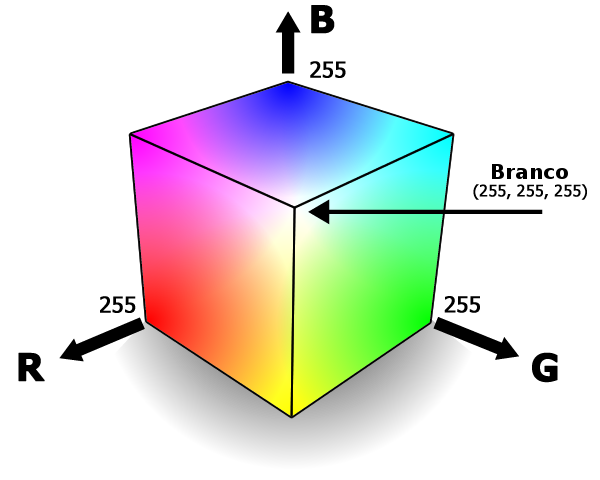
\includegraphics[width=\textwidth,scale=1]{imagens/ex4/rgbColorspace.png}
                \caption{}
                \label{fig:passaBaixa}
        \end{subfigure}%
        ~ %add desired spacing between images, e. g. ~, \quad, \qquad, \hfill etc.
          %(or a blank line to force the subfigure onto a new line)
        \begin{subfigure}[b]{0.3\textwidth}
                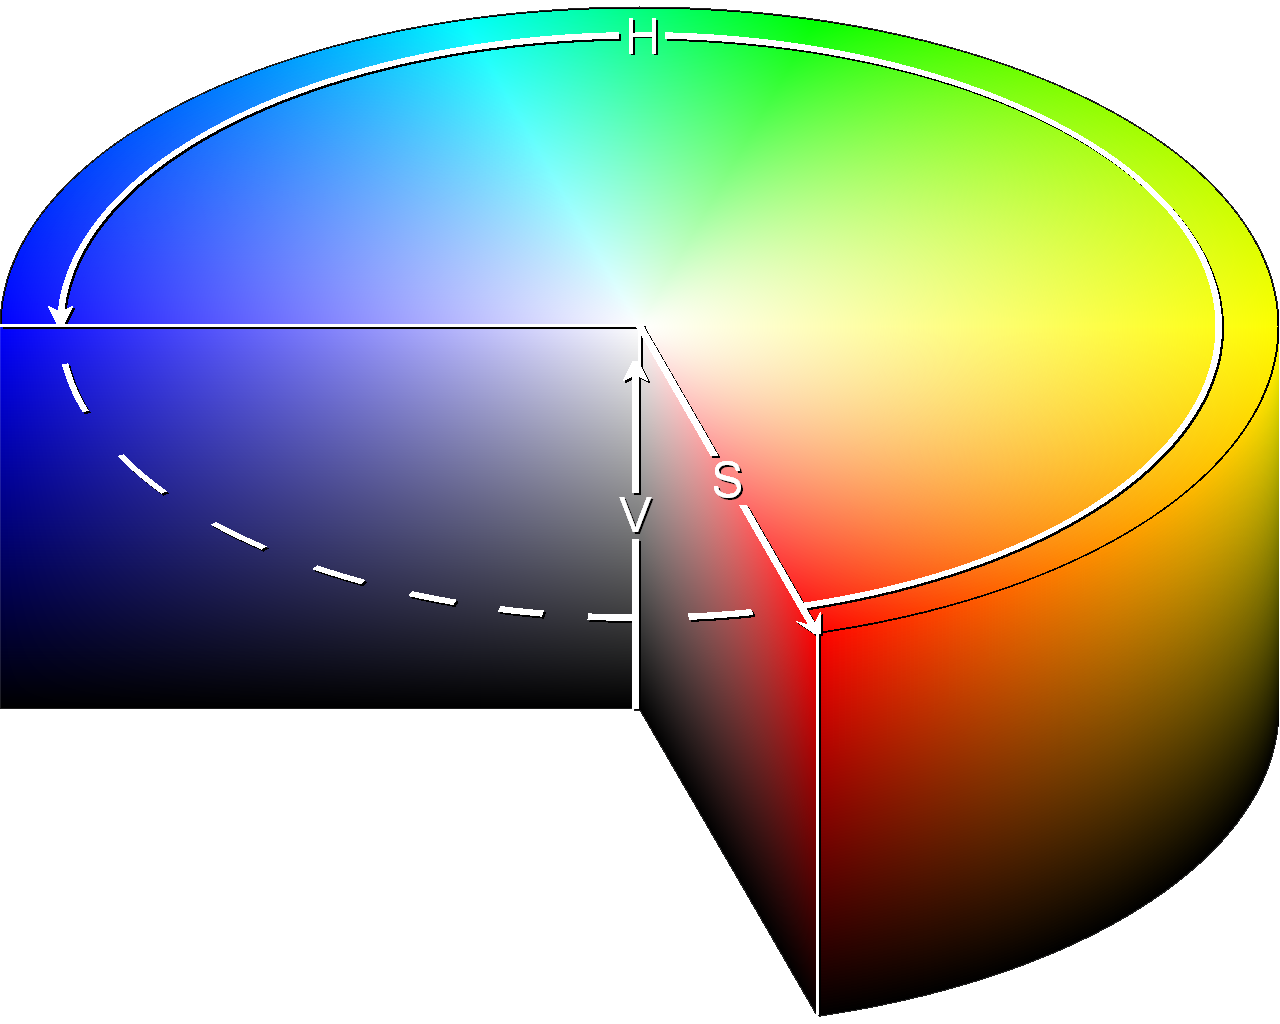
\includegraphics[width=\textwidth,scale=1]{imagens/ex4/HSVColorSpace.png}
                \caption{}
                \label{fig:passaAlta}
        \end{subfigure}
       
        \caption{ 
        \ref{fig:passaBaixa}. Filtro passa baixa.
        \ref{fig:passaAlta}. Filtro passa alta.
        }
	\label{fig:filtrosFrequencia}
\end{figure}

\subsection{Definição do limiar de segmentação}

\subsection{Segmentação baseada na cor da pele}
% ---
% Finaliza a parte no bookmark do PDF, para que se inicie o bookmark na raiz
% ---
\bookmarksetup{startatroot}% 
% ---

% ---
% Conclusão
% ---
\section*{Considerações finais}
\addcontentsline{toc}{section}{Considerações finais}

\lipsum[1]

\begin{citacao}
\lipsum[2]
\end{citacao}

\lipsum[3]
% ]  				% FIM DE ARTIGO EM DUAS COLUNAS
% ---

% ----------------------------------------------------------
% Referências bibliográficas
% ----------------------------------------------------------
\bibliography{pdi}

% ----------------------------------------------------------
% Glossário
% ----------------------------------------------------------
%
% Há diversas soluções prontas para glossário em LaTeX. 
% Consulte o manual do abnTeX2 para obter sugestões.
%
%\glossary

% ----------------------------------------------------------
% Apêndices
% ----------------------------------------------------------

% ---
% Inicia os apêndices
% ---
\begin{apendicesenv}

% ----------------------------------------------------------
\chapter{Nullam elementum urna vel imperdiet sodales elit ipsum pharetra ligula
ac pretium ante justo a nulla curabitur tristique arcu eu metus}
% ----------------------------------------------------------
\lipsum[55-57]

\end{apendicesenv}
% ---

% ----------------------------------------------------------
% Anexos
% ----------------------------------------------------------
\cftinserthook{toc}{AAA}
% ---
% Inicia os anexos
% ---
%\anexos
\begin{anexosenv}

% ---
\chapter{}
% ---

\lipsum[31]

\end{anexosenv}

\end{document}
